\documentclass[tikz,border=2pt]{standalone}
\usepackage{amsmath}
\usepackage{pgfplots}
\pgfplotsset{compat=1.18}
\usetikzlibrary{arrows.meta}
\begin{document}
% Example 2: compact cut disc V (x1^2+x2^2<=9, x1>=-1, x2>=2); Ext(V) = arc from (-1,2sqrt2) to (sqrt5,2) plus (-1,2), and V = Conv(Ext(V)).
% Example 3: closed unbounded W (x1,x2>=0, x1+x2>=1); Ext(W)={(0,1),(1,0)}, Conv(Ext(W)) is a segment that misses (2,2).
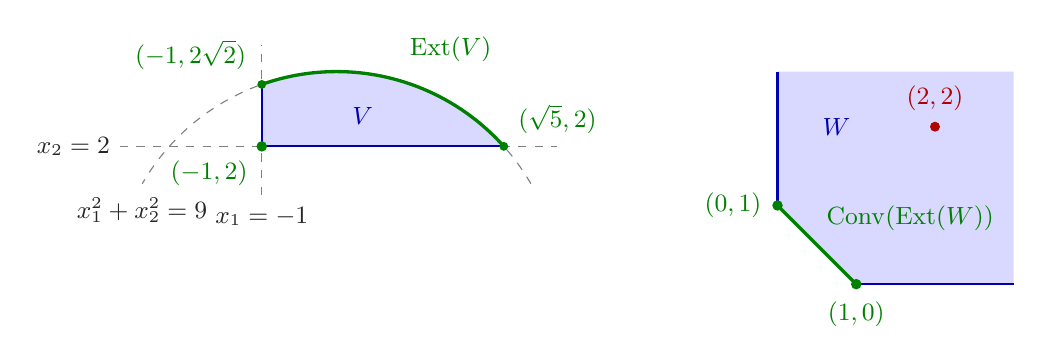
\begin{tikzpicture}[font=\small, >={Latex[length=2mm]}]
  \begin{scope}[x=0.95cm, y=0.95cm]
    \draw[gray, thin, dashed] (30:3) arc[start angle=30, end angle=150, radius=3];
    \draw[gray, thin, dashed] (-1,1.35) -- (-1,3.35);
    \draw[gray, thin, dashed] (-2.9,2) -- (2.95,2);
    \fill[blue!15] (-1,2) -- (-1,{2*sqrt(2)}) arc[start angle=109.47, end angle=41.81, radius=3] -- cycle;
    \draw[blue!70!black, thick] (-1,{2*sqrt(2)}) -- (-1,2) -- ({sqrt(5)},2);
    \draw[green!50!black, very thick] (-1,{2*sqrt(2)}) arc[start angle=109.47, end angle=41.81, radius=3];
    \fill[green!50!black] (-1,2) circle (1.9pt) (-1,{2*sqrt(2)}) circle (1.6pt) ({sqrt(5)},2) circle (1.6pt);
    \node[blue!70!black] at (0.35,2.4) {$V$};
    \node[green!50!black, anchor=north east] at (-1.06,1.94) {$(-1,2)$};
    \node[green!50!black, anchor=south east] at (-1.08,2.9) {$(-1,2\sqrt{2})$};
    \node[green!50!black, anchor=south west] at (2.3,2.04) {$(\sqrt{5},2)$};
    \node[green!50!black, anchor=south west] at (0.85,3.0) {$\operatorname{Ext}(V)$};
    \node[gray!30!black, anchor=north] at (-2.6,1.45) {$x_1^2+x_2^2=9$};
    \node[gray!30!black, anchor=north] at (-1,1.32) {$x_1=-1$};
    \node[gray!30!black, anchor=east] at (-2.9,2) {$x_2=2$};
  \end{scope}
  \begin{scope}[xshift=5.6cm, yshift=0.15cm, x=1cm, y=1cm]
    \fill[blue!15] (0,1) -- (0,2.7) -- (3.0,2.7) -- (3.0,0) -- (1,0) -- cycle;
    \draw[blue!70!black, thick] (0,2.7) -- (0,1) (1,0) -- (3.0,0);
    \draw[green!50!black, very thick] (0,1) -- (1,0);
    \fill[green!50!black] (0,1) circle (1.9pt) (1,0) circle (1.9pt);
    \node[green!50!black, anchor=east] at (-0.08,1) {$(0,1)$};
    \node[green!50!black, anchor=north] at (1,-0.1) {$(1,0)$};
    \node[green!50!black, anchor=south west] at (0.5,0.55) {$\operatorname{Conv}(\operatorname{Ext}(W))$};
    \fill[red!70!black] (2,2) circle (1.8pt);
    \node[red!70!black, anchor=south] at (2,2.08) {$(2,2)$};
    \node[blue!70!black] at (0.75,2.0) {$W$};
  \end{scope}
\end{tikzpicture}
\end{document}
